\documentclass{article}  
\title{algorithm}
\usepackage{CJKutf8}
\usepackage{listings}
\usepackage{amsmath}
\usepackage{amsfonts}
\usepackage{mathtools,amssymb}
\usepackage{graphicx}
\usepackage{mathrsfs}  
\begin{document}

\begin{CJK}{UTF8}{gbsn} 
	在这里我们假设你已经对latex有着一定的了解,并且已经在电脑中装上了相应的texlive和中文字体;\\
	匹配和转录的算法通常遵循所提供的模式或模板的递归结构。 匹配使用模式p来实施与tokens tree序列s的等同性,同时将变量x添加到模式环境Θ中。 Transcribe使用模板t来生成新的语法s,方法是用基于Θ的替换替换所有的自由模式变量x。
\end{CJK}	

\begin{equation}
	match : p * s * \theta \rightarrow (\theta, s);\\
    transcribe : t * \theta \rightarrow s
\end{equation}

\begin{lstlisting}
macro  unless  {
  	rule{ $x $y }=>{ if ( ! $x )  $y }
}
unless (  success ) fail() ;
\end{lstlisting}

\begin{CJK}{UTF8}{gbsn}
	下面给出一个代码,显示了一个简单的匹配和转录的例子,作为宏扩展的一部分。
	
\end{CJK}
$
\\
expand_{\sum} \; ( unless \cdot (success) \quad fail();) \\
\hookrightarrow  match (x \cdot y, (success)fail(); \qquad  \varnothing )\\
\rightarrow match (y, fail() ;,  \qquad[x\mapsto (success)]) \\
\rightarrow match (\epsilon ,;,\qquad[x\mapsto (success),y\mapsto fail()])\\
\hookrightarrow transcribe ( if ( ! x) \cdot y,\qquad[x\mapsto (success),y\mapsto fail()])\\
\rightarrow if (!(success))\quad fail();\\
\\
$

\begin{CJK}{UTF8}{gbsn} 
	完整的算法则如下所示。
\end{CJK}

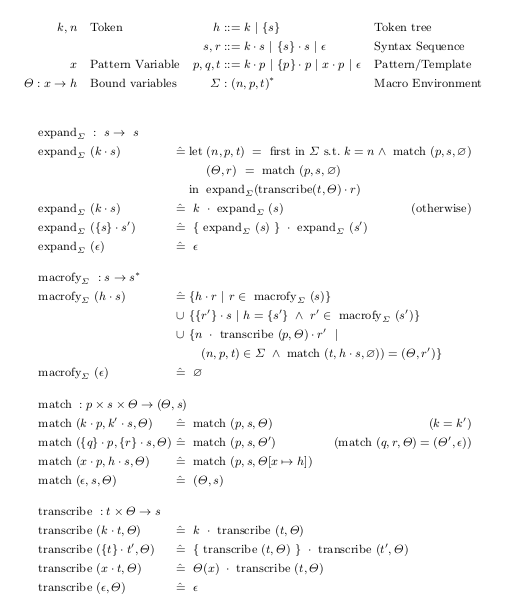
\includegraphics[scale = 0.9]{algorithm.png}
%expand_{\sum} (unless · (success) fail();)
%\hookrightarrow match (x · y, (success) fail();
%\hookrightarrow match (y, fail() ;
%\hookrightarrow match (
%\hookrightarrowtranscribe ( if ( ! x) · y,
%[x 7→ (success)])
%[x 7→ (success), y 7→ fail()])
%[x 7→ (success), y 7→ fail()])
%→ if (!(success)) fail();

\end{document}